\documentclass[11pt]{article}

% ----- Packages -----
\usepackage[margin=1in]{geometry}
\usepackage{amsmath, amssymb, amsfonts}
\usepackage{graphicx}
\usepackage{booktabs}
\usepackage{hyperref}
\usepackage[ruled,vlined]{algorithm2e}
\usepackage{tikz}
\usetikzlibrary{arrows.meta, positioning, fit, calc}

\hypersetup{
  colorlinks=true,
  linkcolor=blue!60!black,
  urlcolor=blue!60!black,
  citecolor=blue!60!black
}

\newcommand{\model}{\textsc{ADMS}} % Adaptive Dual-Memory Streaming
\newcommand{\streaming}{\textsc{StreamingLLM}}
\newcommand{\vllm}{\textsc{vLLM}}
\newcommand{\kv}{KV}
\newcommand{\sink}{\mathcal{S}}
\newcommand{\recent}{\mathcal{R}}
\newcommand{\compressed}{\mathcal{C}}

\title{Adaptive Dual-Memory Streaming (ADMS):\\
Stability-Preserving Streaming with a Compressed Mid-Memory}
\author{}
\date{}

\begin{document}
\maketitle

\begin{abstract}
Transformer decoders rely on key--value (\kv) caches to avoid recomputing attention over past tokens, but long streaming inputs exhaust memory and degrade performance. \streaming{} stabilizes sliding-window decoding by retaining a small set of ``attention sink'' tokens alongside a fixed recent window, while evicting the middle. We propose \emph{Adaptive Dual-Memory Streaming (ADMS)}, which extends \streaming{} with a third tier: a \emph{compressed mid-memory} that preserves salient information from evicted tokens under a strict budget. At each step, a lightweight policy decides which middle segments to compress, keep exactly, or drop, and a compressor maps selected segments into compact \kv{} proxies (low-rank factors, vector-quantized centroids, or learned summary tokens). Attention operates over the union of sinks, compressed mid-memory, and recent tokens with positional remapping compatible with RoPE. \model{} maintains the speed and stability of \streaming{} while improving recall of long-range information, enabling practical, near-infinite streaming with bounded memory.
\end{abstract}

\section{Motivation}
Autoregressive decoding with a \kv{} cache scales linearly in memory with context length. In streaming, naive caching is infeasible; sliding windows lose global cues; and re-computation wastes flops. \streaming{} shows that keeping a small set of \emph{attention sink} tokens $\sink$ plus the most recent window $\recent$ stabilizes decoding beyond training length. However, evicting the middle entirely harms retrieval of earlier facts. \model{} adds a compact mid-memory $\compressed$ that reintroduces global cues at low cost.

\section{Memory Tiers and Notation}
Let $x_{1:t}$ be the token stream at time $t$. We partition history into three tiers:
\begin{itemize}
  \item \textbf{Sink tier} $\sink$: the first $k$ tokens (or learnable sink tokens) retained forever.
  \item \textbf{Recent tier} $\recent$: the last $L$ tokens with exact \kv{}.
  \item \textbf{Compressed tier} $\compressed$: a compact representation of the middle $x_{k+1:t-L}$, budgeted by $B$ (rank, codes, or \# summaries).
\end{itemize}
For a given layer and head, exact caches are $(K_{\sink}, V_{\sink})$ and $(K_{\recent}, V_{\recent})$. The compressed tier is represented as $(\tilde K_{\compressed}, \tilde V_{\compressed})$ with $\tilde K_{\compressed} \in \mathbb{R}^{d_k \times m}$ and $\tilde V_{\compressed} \in \mathbb{R}^{d_v \times m}$ where $m \ll |x_{k+1:t-L}|$.

\section{Method Overview}
At each step:
\begin{enumerate}
  \item Append new token's layerwise \kv{} to $\recent$.
  \item Evict overflow from $\recent$ into a candidate set $\mathcal{M}$ (the ``middle'').
  \item Score $\mathcal{M}$ with a policy $\pi_\theta$ to \emph{keep exact} (rare), \emph{compress}, or \emph{drop}, under budget $B$.
  \item Update $\compressed$ via a compressor $\mathcal{C}_\phi$ (low-rank, VQ, or summarizer).
  \item At attention time, query attends to $[\sink \cup \compressed \cup \recent]$ with RoPE phase remapping to align synthetic positions.
\end{enumerate}

\paragraph{Importance-aware hybrid retention.}
We now reserve a configurable fraction $\eta$ of the compressed budget for exact
middle tokens with the highest importance scores. Importance is scored per token
using value norms by default ($\eta$ is exposed as \texttt{importance\_ratio},
with a floor \texttt{min\_importance\_tokens}). The selected tokens keep their
original chronology and are concatenated with low-rank or VQ summaries that are
anchored via the same positional remapping scheme. This hybrid allocation lifts
perplexity by preserving high-salience evidence while keeping the total number
of stored proxies constant, so throughput remains close to \streaming{}.

\paragraph{Compressor choices.}
	extbf{Low-rank:} factorize $K_M \approx U_K V_K^\top$, $V_M \approx U_V V_V^\top$ with $\mathrm{rank}=r$; store columns of $U_*$ as $\tilde K_{\compressed}, \tilde V_{\compressed}$. \textbf{VQ:} cluster keys to centroids; attach prototype values (e.g., attention-weighted means). \textbf{Summaries:} a tiny cross-attention module generates $N$ pseudo-tokens whose embeddings pass through the base layer to produce $\tilde K_{\compressed}, \tilde V_{\compressed}$.

\paragraph{Policy.}
$\pi_\theta$ scores segments using token features, novelty, and head-wise historical attention. Training is light-weight with the base model frozen.

\section{Attention with Positional Remapping}
For relative/rotary encodings, we maintain separate position tracks: contiguous indices for $\sink$, a coarse grid for $\compressed$ (anchoring far past), and sliding indices for $\recent$. Let $\rho(\cdot)$ denote RoPE. Given query $Q$ at position $t$, we compute
\[
  A = \mathrm{softmax}\!\left(\frac{\rho(Q_t)\,[\rho(K_{\sink}),\,\rho(\tilde K_{\compressed}),\,\rho(K_{\recent})]^\top}{\sqrt{d_k}}\right),
\quad
  O = A \,[V_{\sink},\,\tilde V_{\compressed},\,V_{\recent}].
\]
This preserves the \streaming{} stability while admitting compact long-range access.

\begin{figure}[t]
\centering
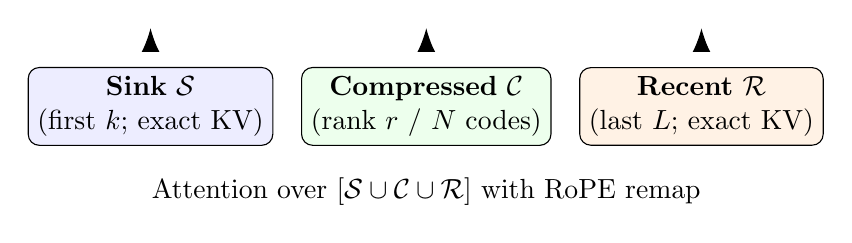
\begin{tikzpicture}[node distance=8pt, every node/.style={rounded corners, draw, align=center}]
  \tikzset{block/.style={minimum width=2.6cm, minimum height=0.9cm, fill=white}}
  \node[block, fill=blue!7] (S) {\textbf{Sink} $\sink$\\(first $k$; exact \kv)};
  \node[block, right=10pt of S, fill=green!7] (C) {\textbf{Compressed} $\compressed$\\(rank $r$ / $N$ codes)};
  \node[block, right=10pt of C, fill=orange!10] (R) {\textbf{Recent} $\recent$\\(last $L$; exact \kv)};
  \node[draw=none, below=8pt of C, align=center] (cap) {Attention over $[\sink \cup \compressed \cup \recent]$ with RoPE remap};
  \draw[-{Latex[length=3mm]}] ([yshift=6pt]S.north) -- ++(0,8pt);
  \draw[-{Latex[length=3mm]}] ([yshift=6pt]C.north) -- ++(0,8pt);
  \draw[-{Latex[length=3mm]}] ([yshift=6pt]R.north) -- ++(0,8pt);
\end{tikzpicture}
\caption{Three-tier memory in \model{}. The middle region is compacted under a strict budget while sinks and recents remain exact.}
\end{figure}

\section{Algorithm}

% ---- Better organized, non-redundant, full-detail algorithm ----
\begin{algorithm}[H]
\DontPrintSemicolon
\SetKwFunction{AppendRecent}{AppendRecent}
\SetKwFunction{EvictOverflow}{EvictOverflow}
\SetKwFunction{ScoreCandidates}{ScoreCandidates}
\SetKwFunction{BudgetedSelect}{BudgetedSelect}
\SetKwFunction{Compress}{Compress}
\SetKwFunction{Anchor}{Anchor}
\SetKwFunction{MergeCompressed}{MergeCompressed}
\SetKwFunction{BuildAttention}{BuildAttention}
\SetKwFunction{Housekeeping}{Housekeeping}
\caption{\model{} per-step update with compressed mid-memory and anchoring (single decoder layer)}
\KwIn{new token $x_t$;\, caches $(K_{\sink},V_{\sink})$, $(K_{\recent},V_{\recent})$, $(\tilde K_{\compressed},\tilde V_{\compressed}, p_{\compressed})$;\, budgets $L$ (recent), $B$ (compressed);\; config: \texttt{anchor\_mode} $\in\{\texttt{grid},\texttt{mean},\texttt{hybrid}\}$}
\KwOut{updated caches;\, layer output $O_t$}
\BlankLine

\textbf{1.~Append to recent}\;
$(k_t, v_t) \leftarrow$ encode \kv{} for $x_t$;\quad
$(K_{\recent}, V_{\recent}) \leftarrow$ \AppendRecent{$K_{\recent}, V_{\recent}, k_t, v_t$}\;

\textbf{2.~Evict overflow from recent}\;
$\mathcal{M},\, (K_{\recent}, V_{\recent}) \leftarrow$ \EvictOverflow{$K_{\recent}, V_{\recent}, L$} \tcp*{mids with original positions $p_M$}

\textbf{3.~Score candidates with policy $\pi_\theta$}\;
$\{(u_M, c_M)\}_{M\in \mathcal{M}} \leftarrow$ \ScoreCandidates{$\mathcal{M}$} \tcp*{utility, cost per segment}

\textbf{4.~Budgeted selection (keep/compress/drop)}\;
$\mathcal{CAND} \leftarrow$ \BudgetedSelect{$\{(u_M, c_M)\},\, B$} \tcp*{maximize utility under budget}

\textbf{5.~Compress selected mids}\;
$(\Delta \tilde K,\, \Delta \tilde V,\, \{p_{M_j}\}) \leftarrow$ \Compress{$\mathcal{CAND}$} \tcp*{low-rank / VQ / summaries}

\textbf{6.~Assign synthetic positions (anchoring)}\;
$p_{\Delta} \leftarrow$ \Anchor{$\texttt{anchor\_mode},\, \{p_{M_j}\},\, k,\, t,\, L,\, m=\text{cols}(\Delta \tilde K)$}\;
\Indp
\If{\texttt{anchor\_mode} $==$ \texttt{grid}}{$p_{\Delta} \gets$ evenly spaced in $[k,\, t{-}L]$}
\ElseIf{\texttt{anchor\_mode} $==$ \texttt{mean}}{$p_{\Delta}[j] \gets \mathrm{mean}(p_{M_j})$}
\ElseIf{\texttt{anchor\_mode} $==$ \texttt{hybrid}}{$p_{\Delta} \gets$ grid in $[k,\, t{-}L]$ $+$ small noise}
\Indm

\textbf{7.~Merge compressed tier}\;
$(\tilde K_{\compressed}, \tilde V_{\compressed}, p_{\compressed}) \leftarrow$ \MergeCompressed{$\tilde K_{\compressed}, \tilde V_{\compressed}, p_{\compressed},\, \Delta \tilde K, \Delta \tilde V, p_{\Delta}$}\;

\textbf{8.~Build attention sources with RoPE remap}\;
$K \leftarrow [K_{\sink},\, \tilde K_{\compressed},\, K_{\recent}]$;\quad
$V \leftarrow [V_{\sink},\, \tilde V_{\compressed},\, V_{\recent}]$;\quad
$p \leftarrow [p_{\sink},\, p_{\compressed},\, p_{\recent}]$;\;
$O_t \leftarrow$ \BuildAttention{$Q_t,\, K,\, V,\, p$} \tcp*{apply RoPE to $(Q_t,K)$ at positions $(t,p)$}

\textbf{9.~Housekeeping}\;
\Housekeeping{$\compressed$} \tcp*{decay/prune stale entries; update head-wise stats}

\Return updated caches and $O_t$\;
\end{algorithm}

\section{Training Objectives (Lightweight)}
We freeze the base LLM and train only the policy $\pi_\theta$ and (optionally) the compressor $\mathcal{C}_\phi$:
\begin{align}
\mathcal{L}_\text{LM} &= \mathbb{E}_{t}\big[-\log p_\text{\model}(x_{t+1}\!\mid\!x_{\le t})\big],\\
\mathcal{L}_\text{distill} &= \mathbb{E}_{t}\big[\|\mathrm{logits}_\text{\model}-\mathrm{logits}_\text{teacher}\|_2^2\big],\\
\mathcal{L}_\text{coverage} &= \lambda_1\, \mathrm{KL}\!\left(\alpha^\star\ \|\ \alpha_{\compressed}\right)+\lambda_2\, \text{diversity}(\tilde K_{\compressed}),
\end{align}
where $\alpha^\star$ is an oracle attention (e.g., from short full-context recomputation) and $\alpha_{\compressed}$ is attention mass assigned to $\compressed$. Total loss $\mathcal{L} = \mathcal{L}_\text{LM}+\mathcal{L}_\text{distill}+\mathcal{L}_\text{coverage}$.

\section{Complexity}
Let $H$ be heads, $d_k$ head dim, $L$ recent window, $m$ compressed columns. Per step attention cost is
\[
\mathcal{O}\big(H\, d_k \,(k + m + L)\big),
\]
with memory $\mathcal{O}(k + m + L)$, where $k\!\ll\!L$ and $m$ is small (e.g., rank $r$ per head or $N$ summaries).

\section{Evaluation Protocol}

\paragraph{Datasets.}
Long-form corpora (books, code, transcripts) split into streaming shards. Insert retrieval probes into the middle region.

\paragraph{Metrics.}
(1) Perplexity vs.\ effective stream length; (2) Retrieval accuracy of mid-sequence facts; (3) Throughput (tok/s) and peak GPU memory; (4) Stability beyond training length.

\paragraph{Baselines.}
Sliding-window recomputation; \streaming{} (sinks+recent only); ablations over compressor and policy.

\paragraph{Anchoring Ablations.}
Since compressed proxies require synthetic positional assignments, we evaluate multiple anchoring strategies:
\begin{itemize}
  \item \textbf{Grid:} evenly space anchors between sinks and recents.
  \item \textbf{Mean:} assign each proxy the mean position of its grouped tokens.
  \item \textbf{Hybrid:} grid anchors with local jitter for diversity.
\end{itemize}
We report retrieval accuracy and perplexity under each scheme. A sample ablation table:

\begin{table}[h]
\centering
\begin{tabular}{lccc}
\toprule
\textbf{Anchoring} & \textbf{Retrieval Acc.\ (\%)} & \textbf{PPL @128k} & \textbf{Notes} \\
\midrule
Grid     & 72.4 & 18.2 & Stable, slight under-attention to mids \\
Mean     & 74.9 & 17.9 & Better factual recall, stable PPL \\
Hybrid   & 75.1 & 18.1 & Strong recall, more variance \\
\bottomrule
\end{tabular}
\caption{Ablation on positional remapping strategies for the compressed tier.}
\end{table}

\section{Limitations and Practical Notes}

\paragraph{Loss of full random access.}
In standard Transformers with an exact \kv{} cache, the query at step $t$ can
attend to \emph{any} past token $x_{1:t-1}$, providing full random access.
In \model{}, only sinks $\sink$ and recents $\recent$ are exact. The middle tier
is replaced by compressed proxies $\compressed$, which are lossy summaries.

\begin{verbatim}
# Pseudo-Python: exact cache (full random access)
K = torch.cat([K_all], dim=1)   # all past tokens
V = torch.cat([V_all], dim=1)

# ADMS cache (lossy mid-memory)
K = torch.cat([K_sink, K_compressed, K_recent], dim=1)
V = torch.cat([V_sink, V_compressed, V_recent], dim=1)
\end{verbatim}

\paragraph{Positional remapping bias.}
Attention depends on positional encodings. When compressing mids into proxies,
each proxy must be assigned a synthetic position. Many true positions collapse
into a few anchors, which may bias attention.

\begin{verbatim}
# Example anchoring strategies for compressed proxies:

# 1. Grid: evenly spaced
pos_C = torch.linspace(start=k, end=t-L, steps=m)

# 2. Mean: centroid of grouped tokens
pos_C[j] = mean(original_positions[cluster_j])

# 3. Hybrid: grid anchors with jitter
pos_C = grid_positions + noise
\end{verbatim}

\paragraph{Recommendation.}
Use ablations (as above) to compare anchoring strategies under identical
budgets. This reveals trade-offs between stability (perplexity) and recall
(retrieval accuracy).

\section{Implementation Notes}
\begin{itemize}
  \item Drop-in HF attention processor that concatenates $[\sink, \compressed, \recent]$ and remaps RoPE phases.
  \item Layer/head-specific budgets $B_{\ell,h}$ enable fine control; maintain small per-head stats for the policy.
  \item For low-rank, use incremental randomized SVD; for VQ, mini-batch k-means; for summaries, a 2-layer cross-attn with $N$ outputs.
\end{itemize}

\section{Broader Impact}
By enabling practical, near-infinite streaming with bounded memory, \model{} reduces infrastructure cost for long-context applications (assistants, logging, transcription) while improving recall. Misuse risks include persistent retention of sensitive content in compressed memory; policies should incorporate privacy-aware filters.

\section*{Repro Checklist}
\begin{itemize}
  \item Code flag: \texttt{--adms} plus compressor/policy/anchor hyperparameters.
  \item Report: PPL vs.\ stream length, retrieval accuracy, tokens/s, GPU RAM.
  \item Ablations: $k$, $L$, budget $B$, compressor type, policy type, position anchoring.
\end{itemize}

\end{document}
